\documentclass{thesis}

% TX Fonts を使う
\usepackage{txfonts}

%アルゴリズムパッケージを使用

\usepackage{algorithm}
\usepackage{algorithmic}
\usepackage{listings, jlisting}

\usepackage{ascmac,here,txfonts,txfonts}
\usepackage{listings,jlisting}
\usepackage{color}

\lstset{
  breaklines = true,
  language=java,
  basicstyle=\ttfamily\scriptsize,
  commentstyle={\itshape \color[cmyk]{1,0.4,1,0}},
  classoffset=1,
  keywordstyle={\bfseries \color[cmyk]{0,1,0,0}},
  stringstyle={\ttfamily \color[rgb]{0,0,1}},
  frame=tRBl,
  framesep=5pt,
  showstringspaces=false,
  numbers=left,
  stepnumber=1,
  numberstyle=\tiny,
  tabsize=2,
}

\begin{document}

% 目次
\tableofcontents
%%%%%%%%%%%%%%%%%%%%%%%%%%%%%%%%%%%%%%%%%%%%%%%%%%%%%%%%%%%%%%%%%%%%%%%%%%%%%%%%%%%%%%%%%%%%%%%%%%%%%%%%%%%%%%%%%%%%%%

\chapter{序論}

QRコード\cite{QR}は、1994年に株式会社デンソーウェーブが開発した二次元バーコード であり、食品や交通分野など多方面の分野で利用されている.
白と黒の正方形のモジュールから構成され、ランダムな見た目で表される.
一般的なQRコードはデザイン性を考慮していないが、一方で広告、サービス業界ではデザイン性を考慮したQRコードが求められている.
デザイン性を考慮したQRコードでは、一定のルールからQRコードを変更することによって、QRコード上にロゴ画像(以後、目的画像と述べる)を埋め込んだものがある.
このようなQRコードをAesthetic QRコード\cite{KURI}という.

Aesthetic QRコードの研究は大きく三種類に分けることができる.

\begin{enumerate}
\item
QRコードの一部に目的画像を埋め込む方法.
\item
画像のヒストグラムを考慮して目的画像を埋め込む方法\cite{hist}.
\item
RS符号のパディングビットを考慮して目的画像を埋め込む方法\cite{KURI}.
\end{enumerate}

本研究は、上に述べた三つ目に分類されるRS符号のパディングビットを考慮して目的画像を埋め込む方法を考察し、目的画像に近いAesthetic QRコードを自動生成する方法について検討する.
Aesthetic QRコードを自動生成する手法として、本研究では、Kuribayashiらの論文\cite{KURI}で提案されているランダム手法のアルゴリズムを用い、Aesthetic QRコードを生成するソフトウェアを開発することを研究の目的とする.

以下、第\ref{chap:2}章ではQRコードを構成するReed-Solomon符号とQRコードの概要について述べ、第\ref{chap:3}章では本研究のベースとなっているKuribayashiらの論文\cite{KURI}のランダム法について述べる.
第\ref{chap:4}章では実験により得られた結果について述べる.
第\ref{chap:5}章では結論と今後の課題について述べる.


%%%%%%%%%%%%%%%%%%%%%%%%%%%%%%%%%%%%%%%%%%%%%%%%%%%%%%%%%%%%%%%%%%%%%%%%%%%%%%%%%%%%%%%%%%%%%%%%%%%%%%%%%%%%%%%%%%%%%%%%%
\chapter{QRコード}
\label{chap:2}

\section{Reed-Solomon符号}

Reed-Solomon符号(以下、RS符号)は誤り訂正符号の一つであり、有限体や拡大体上で実装される.その誤り訂正能力は高くQRコードでも応用されている.
付加した符号を用いることで誤りを検知でき、決められた数以下のノイズであれば誤りを訂正できる.

拡大体$GF(p^j)$上において、符号のデータは複数のビットを1つのデータ単位として扱い、このデータ単位のことをシンボルと呼ぶ.

RS符号はRS符号の符号長を$n$シンボル、シンボル・エラー訂正最大数を$d$個、データ長を$k$シンボルと置くとき、$(n,k)$符号と呼ぶ.
RS符号のデータ長$k$シンボルはデータ部と呼ぶ.データ長$n-k$シンボルはパリティ部と呼び、誤り訂正に使われる.


RS符号のデータ部は固定長である.QRコードに入れる文字列が既定の数より少ない場合、データ部の係数を所定の数に合わせるためパディングビット(埋め草コード)を付加する.
入力データをRS符号の係数に落とし込んだ時の個数を$\hat{k}$と表すとき、\\
入力データ部分を表すRS符号の係数は

\begin{equation}
\alpha_{\hat{k}},…,\alpha_1
\label{eq:pol1}
\end{equation}

である.$\hat{k} < k$の時、RS符号のデータ部の係数を$k$個に合わせるため、パディングビットを付加する.
これにより、RS符号のデータ部の係数は

\begin{center}
$\alpha_{k},…,\alpha_{\hat{k} + 1},\alpha_{\hat{k}},…,\alpha_1$
\end{center}
と表す.
なお、パディングビットは
 
 \begin{equation}
 \alpha_{k},…,\alpha_{\hat{k} + 1}
\label{eq:pol3}
\end{equation}
と表す.\\

\newpage

RS符号の全体図を図\ref{RScode}に示す.

\begin{figure}[H]
 \centering
 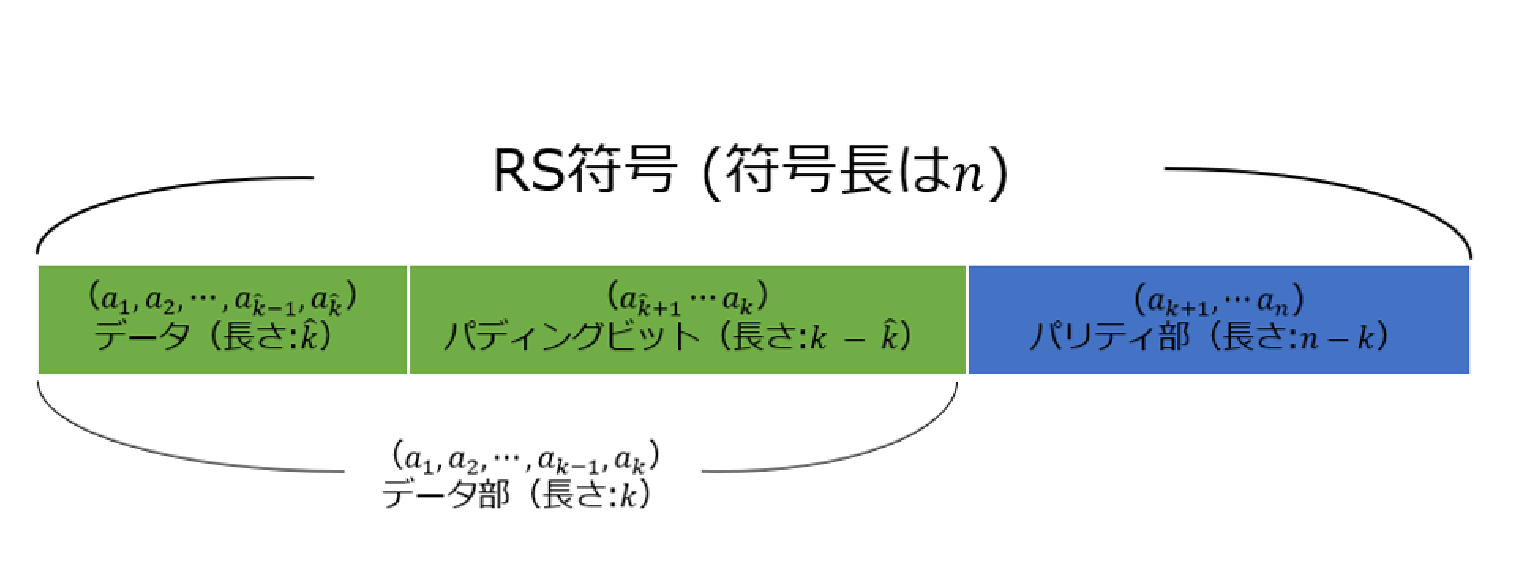
\includegraphics[width=1\linewidth]{pic/RScode.eps}
 \caption{RS符号の全体図\label{RScode}}
\end{figure}

パディングビットはQRコードに入力するデータとは関係ないため、自由に変更できる.
パディングビットを変更することにより、RS符号を形成する多項式の係数は変わる.
そのため、RS符号化で得られる符号の値も変化する.



計算は有限体や拡大体で行われる.符号で用いられる値は原始多項式の元$\alpha$で定義される.
符号を特定するには$n,k$以外に、生成多項式\cite{Ikeda}\cite{Tom}と呼ばれる$n-k$次多項式$g(x)$を選ぶ必要がある.\\
QRコードでは、

\begin{equation}
 g(x)=(x-1)(x-\alpha)\cdots(x-\alpha^{n-k-1})= \prod_{i=0}^{n-k-1}(x-\alpha^i)
 \label{gx}
\end{equation}
であり、式\ref{gx}の$g(x)$を展開した多項式を
\begin{equation}
 g(x)=g_1x^{n-k}+g_2x^{n-k-1}+\cdots+g_{n-k+1},\ g_1=1
 \label{gx_ten}
\end{equation}
とする.その係数列$g_1=1,g_2,\cdots,g_{n-k1}$から定まる$k\times n$行列

\[
  G_0 = \left[
    \begin{array}{cccccccc}
      1        & g_2      & \ldots  & g_{n-k-1} & 0            & \ldots  & \ldots    & 0 \\
      0        & 1        & g_2      & \ldots     & g_{n-k-1}  & 0        & \ldots    & 0 \\
      \vdots & \ddots & \ddots & \ddots     & \ddots     & \ddots & \ddots   & \vdots \\
      0        & \cdots & 0        & 1            & g_2          & \ldots & g_{n-k-1} &       0       \\
      0        & \cdots & \cdots & 0            & 1            & g_2     & \ldots     & g_{n-k-1}       \\
    \end{array}
  \right]
\]
を生成行列と呼ぶ.組織符号を得るには、行列$G_0$を"掃き出し法"によって$G=[I_k,P]$\\
$(I_kはk\times k単位行列)$という標準形に変形する.

RS符号は次のようにして得ることができる.
データ$u$に対する符号語$v$は標準形の生成行列$G=[I_k,P]$により、
\begin{equation}
 v=uG
\end{equation}
として表現することができる.


%RS符号の計算を行う拡大体が$GF(p^j)$上では、原始多項式$G(x)$は次のようになる
%\begin{equation}
%G(x)=x^{j} + b_jx^{j-1} + \cdots + b_1x^1  + 1= 0 
%\label{eq:genshi}
%\end{equation}

%ここで$b_{j},\cdots,b_1\in GF(p^j)$である.\\

%データである$k$シンボルを係数に持つ多項式は情報多項式と定義する.
%これは
%\begin{equation}
%F(x)= \alpha_{n}x^{n-1}+\alpha_{n-1} x^{n-2}+…+\alpha_{2d + 1} x^{2d}
%\label{eq:stainf}
%\end{equation}
%のように表すことができる.
%ここで$a_{n},\cdots,a_{2d+1}\in GF(p^j)$である.\\
%RS符号の生成多項式は$d$個のシンボル・エラーを訂正でき、連続した$\alpha$のべき乗での$2d$個の根を持つ.

%\begin{equation}
%g(x) = (x-\alpha^1)( x-\alpha^2)\cdots( x-\alpha^{2d})
%\label{eq:stagen}
%\end{equation}
 %符号化によって生成するパリティ符号の数は$2d$シンボルであり、パリティ部は$n-k$シンボルであるため、
%\begin{equation*}
%2d=n-k
%\end{equation*}
%が成り立つ.

%%%%%%%%%%%ここからあやしい%%%%%%%%%%%(行列でRS符号化する方法をかくべき)

%符号化は情報多項式を生成多項式で割り、その余りを計算して情報多項式に加えることである.
%RS符号化によって計算された余りは$F(x)$を$g(x)$で割った際にできるものであるため最大次数が$2d - 1$となり、それをパリティ多項式$a(x)$と表す.

%\begin{equation}
%F(x) \bmod g(x) = a(x) = \alpha_{2d}x^{2d - 1}+\cdots + \alpha_1
%\end{equation}

%ここで$a_{2d},\cdots,a_{1}\in GF(p^j)$である.\\
%有限体、拡大体上での演算はXOR演算で行われ、情報多項式にパリティ多項式を足すことにより、情報多項式の余り部分が消える.
%そのため、情報多項式は生成多項式で割り切れるようになる.

%情報多項式とパリティ多項式の和$F(x)+a(x)$は
%\begin{equation}
%F(x)+a(x)= \alpha_{n} x^{n-1}+\alpha_{n-1}x^{n-2}+…+\alpha_1 
%\label{eq:pol}
%\end{equation}
%と表すことができ、これを$R(x)$と定義する.
%この$R(x)$の係数がRS符号である.

%%%%%%%%%%%%%%%%%%%%%%%%%%%%%%%%%%%%%%%


\section{QRコードの概要}

QRコードの構成要素の最小単位は白と黒で表されるモジュールであり、各モジュールには単一ビット値が割り当てられる.
QRコードのサイズはバージョンによって決定され、そのバージョン($v$)は$1\sim40$である.
$1$型は、$21\times21$モジュール、$2$型は、$25\times25$モジュール、というように、型番が一つ上がるごとに一辺につき$4$モジュールずつ増加し、$40$型は、$177\times177$モジュールとなる.
したがって、バージョン$v$は$(17+4v)\times(17+4v)$モジュールである.

図\ref{fig:qrcode_config}にQRコードの構成要素を表す. \\

\begin{figure}[H]
\centering
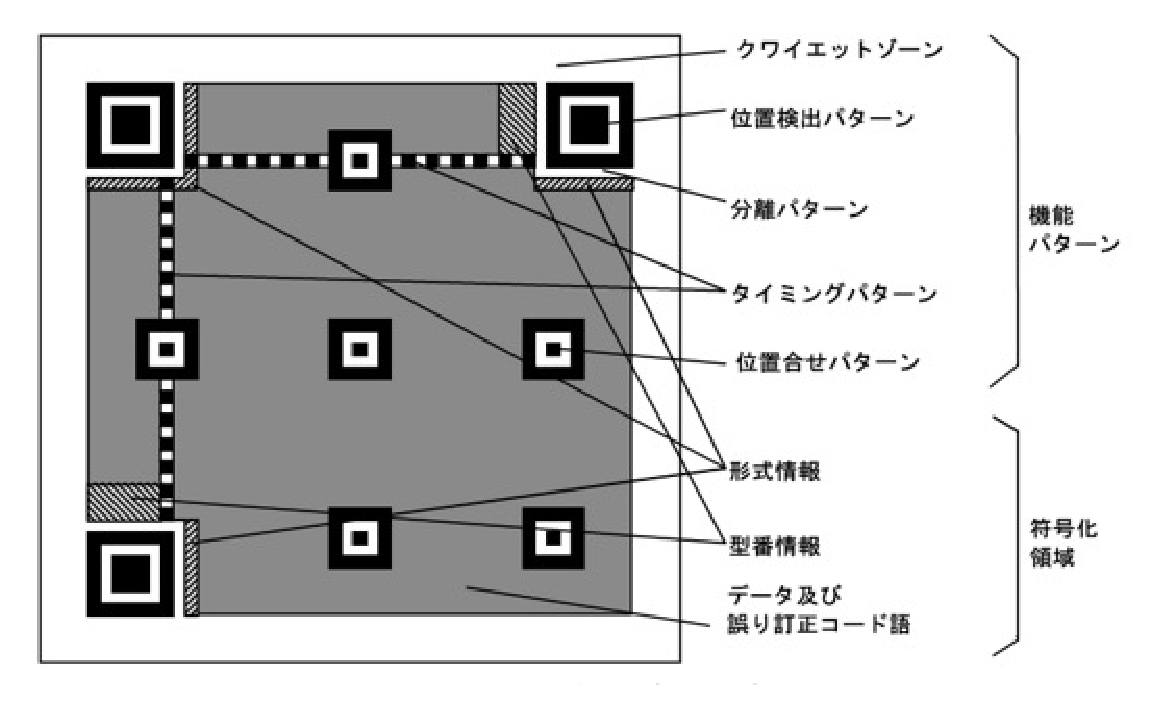
\includegraphics[width=10cm,clip]{pic/qrcode_config.eps}
\caption{QRコードシンボルの構造\cite{jis}}
\label{fig:qrcode_config}
\end{figure}

QRコードは、QRコード上にある符号化されたデータを正確に認識するために機能パターンを持っている.
機能パターンは主に3つの構成要素から成り立っており、それぞれ位置検出パターン、位置合わせパターン、タイミングパターンと呼ばれる.

位置検出パターンはQRコードの左上、左下、右上の角にある3つの正方形のブロックである.
それらの境目を明白にするために、形式情報との間に白いモジュールを置く.これを分離パターンと呼ぶ.

位置合わせパターンは小さな正方形のブロックで、位置検出パターンの垂直・平行座標に関係する位置に置く.バージョンによっては付加しない場合もあり、バージョン1には存在しない.

タイミングパターンは左上の位置検出パターンから右上の位置検出パターンへと、左上の位置検出パターンから左下の位置検出パターンへの白黒が交互に並ぶ$2$つのラインのことである.

QRコードのデータビットは、QRコードの右下から始まり、2モジュール幅の列上に配置する.列が最上部に達すると、次の2モジュール列は右端から始まり、下方向へ続く.現在の列が端に達すると、次の2モジュールの列に移動して方向を変更する.データビットは機能パターン(位置検出パターン、タイミングパターン、位置合わせパターン)の位置では、次のモジュールへ配置される.

上方向のデータビットの配置は表\ref{up_bit}に、下方向のデータビットの配置は表\ref{down_bit}に示す.

\begin{table}[h]
 %---- 最初の表 ---------------------------
  \begin{minipage}[t]{.45\textwidth}
    \begin{center}
	\caption{上方向のビット配列 \label{up_bit}}
      \begin{tabular}{|c|c|} \hline
	0&1\\ \hline
	2&3\\ \hline
	4&5\\ \hline
	6&7\\ \hline
      \end{tabular}
    \end{center}
  \end{minipage}
  %
  \hfill
  %
 %---- 2つ目の表 ---------------------------
  \begin{minipage}[t]{.55\textwidth}
    \begin{center}
	\caption{下方向のビット配列 \label{down_bit}}
      \begin{tabular}{|c|c|} \hline
	6&7\\ \hline
	4&5\\ \hline
	2&3\\ \hline
	0&1\\ \hline
      \end{tabular}
    \end{center}
  \end{minipage}
\end{table}

QRコードは、誤り訂正にRS符号を使用し、その能力はL、M、Q、Hの$4$つのレベルに昇順で分類される.
各誤り訂正レベルはQRコード内の全シンボルの約$7\%$、約$15\%$、約$25\%$、約$30\%$までのシンボルを訂正することができる.
それぞれを表\ref{Correction_ability}に示す.

\begin{table}[htbp]
\begin{center}
  \caption{誤り訂正レベル \label{Correction_ability}}
    \begin{tabular}{|c|c|c|c|c|} \hline
     レベル&L&M&Q&H\\ \hline\hline
     誤り訂正能力&約$7\%$&約$15\%$&約$25\%$&約$30\%$ \\ \hline
    \end{tabular}{}
\end{center}
\end{table}


%%%%%%%%%%%%%%%%%%%%%%%%%%%%%%%%%%%%%%%%%%%%%%%%%%%%%%%%%%%%%%%%%%%%%%%%%%%%%%%%%%%%%%%%%%%%%%%%%%%%%%%%%%%%%%%%%

\chapter{Aesthetic QRコード}
\label{chap:3}

本章では、QRコード上に配置された二値配列が埋め込む目的画像のモジュールパターンと類似した、より埋め込む画像に近いQRコードを得るために用いたKuribayashiらの論文\cite{KURI}のランダム法について述べる.

Aesthetic QRコードを作成するにあたり、本研究ではQRコードに埋め込む画像を目的画像と定義する.

Aesthetic QRコードの例を図\ref{As}に示す.

\begin{figure}[H]
      \centering
      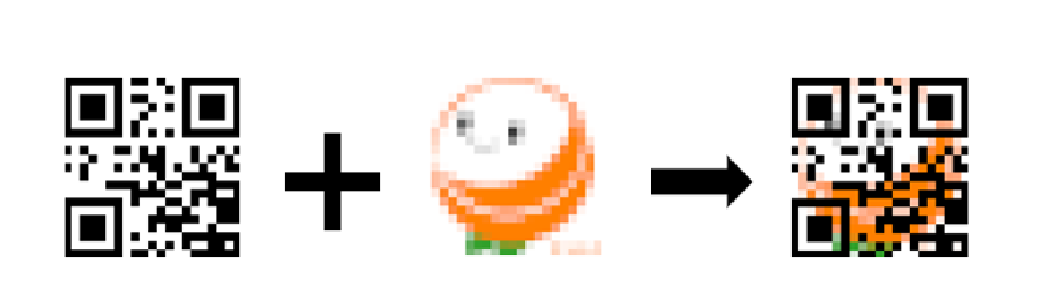
\includegraphics[width=0.7\linewidth]{pic/As.eps}
      \caption{Asethetic QRコード例}
      \label{As}
\end{figure}



\section{色変換手法}

%ここの説明を変える

ランダム法を使用する際に目的画像を二値化してQRコードとのハミング距離を測り、最もハミング距離の小さいQRコードを用いてAesthetic QRコードを作る.
目的画像を二値化画像にする際に閾値を指定するが、その閾値をAlgorithm 1に示す色変換手法で決定する.


\begin{algorithm}                      
\caption{論文\cite{KURI}の色変換手法}         
\label{alg:alg1} 
\begin{description}
\item[入力:] サイズ$L \times L$の目的画像
\item[出力:] 閾値 $\overline{Y}$
\item[方法:]
\begin{enumerate}
\item 入力画像の大きさは、QRコードのバージョン$v$と同じサイズに予め変更しておく.RGB色成分はYUV色成分に変換され、輝度(Y)成分$Y_{i,j}$,($1 \leq i,j \leq L$)が得られる.
\item その中心の正方形(元の画像サイズの$\frac{1}{4}$)の値の平均$\overline{Y}$が計算する.
\begin{equation}
\overline{Y} = \frac{4}{L^2} \sum_{i = \frac{L}{4}}^{\frac{3L}{4} - 1} \sum_{j = \frac{L}{4}}^{\frac{3L}{4} - 1} Y_{i,j}
\label{eq:pol4}
\end{equation}
\end{enumerate}
\end{description}
\end{algorithm}  

閾値を用いて目的画像から目的画像の二値行列を作成するアルゴリズムをAlgorithm 2に示す.

\begin{algorithm}                      
\caption{目的画像に対する二値行列の生成}         
\label{alg:alg2} 
\begin{description}
\item[入力:] サイズ$L \times L$の目的画像の輝度(Y)成分$Y_{i,j}$($1 \leq i,j \leq L$)、閾値$\overline{Y}$
\item[出力:] 二値行列$B_{i,j}$
\item[方法:]
\begin{enumerate}
\item 目的画像を二値化する際、二値行列$B_{i,j}$は、以下の規則によって決定される.
\begin{equation}
{B_{i,j} =}
\begin{cases}
1 & Y_{i,j} > \overline{Y} \\
0 & otherwise 
\end{cases}
\label{eq:binary}
\end{equation}
\end{enumerate}
\end{description}
\end{algorithm} 



\newpage
\section{ランダム法}

%%%%%%%%%%%%%%%%%%%%%%%%%%(ここの説明を詳しくしたい)
ランダム法では、QRコードと目的画像の画像サイズを等いものとして、QRコードの$1$モジュールと目的画像の$1$画素を対応させる.
目的画像とQRコードとの違いを導き出すための手順として、目的画像の二値化を行い、QRコードと二値行列とのハミング距離を取ることを行う.

RS符号化を行う際、掃き出し法により$G$を($I|P)$の形に変形せず後、$I$の後半の列(パティングビット)を$P$のどこかの列に入るように掃き出し法を行う.
試行回数$N$回ランダム法を行い、目的画像に一番近いQRコードを計算する.
目的画像の二値化画像と生成されたQRコードのハミング距離を取り、ハミング距離が最小になるQRコードを使ってAesthetic QRコードを作成する.

\newpage
本研究ではQRコードの中でバージョン1のQRコードを用いた.
バージョン1のQRコードを作成する手順を以下に説明する.

\begin{algorithm}                      
\caption{ランダム法を用いたバージョン1のAesthetic QRコード}         
\label{alg:alg3} 
\begin{description}
\item[入力:] バージョン$1$のQRコードに入る範囲内の文字列、サイズ$21 \times 21$の目的画像
\item[出力:] サイズ$21 \times 21$のバージョン$1$のAesthetic QRコード
\item[方法:]
\begin{enumerate}
\item
目的画像の画素値をQRコードのモジュールに割り当て、Algorithm2で決まった閾値$\overline{Y}$でモジュールを二値化し、二値行列$B_{i,j}$を作成する.
\item
$B_{i,j}$に所定のマスキングパターンを作用させる.
\item
式(\ref{eq:pol3})の$\alpha_{t}$ ($\hat{k} + 1 \leq x_t \leq n $)を変化させることにより、RS符号を見つける.
以後この手順を$N$回繰り返すことにより、$B_{i,j}$とのハミング距離が最小となるRS符号を見つける.
一定の試行回数終了後、QRコード上のRS符号は、最良のRS符号に置き換える.
\item
マスク処理前であるQRコードの各モジュールに対して、所定のマスクパターンを適用する.
\item
目的画像とQRコードをかさねてAethetic QRコードを作成する.
\end{enumerate}
\end{description}
\end{algorithm} 


%%%%%%%%%%%%%%%%%%%%%%%%%%%%%%%%%%%%%%%%%%%%%%%%%%%%%%%%%%%%%%%%%%%%%%%%%%%%%%%%%%%%%%%%%%%%%%%%%%%%

\chapter{バージョン1のAesthetic QRコードのソフトウェア実装と評価}
\label{chap:4}

\section{実験環境}

実験に使用したPC環境、言語を以下に示す.

\begin{itemize}
\setlength{\itemsep}{5mm}
 \item ソフトウェア実装環境
    \begin{itemize}
      \item CPU:Intel(R)Core(TM) i7-7700 CPU @ 3.60GHz 3.60GHz
      \item OS:Windows 10 pro
      \item 実装RAM:16.0GB
     \end{itemize}
   \item 開発環境
    \begin{itemize}
      \item Java:Eclipse 4.11.0
      \item Maple:Maple 2017.3
   \end{itemize}
\end{itemize}

実験に使用した各パラメータを以下に示す.

\begin{itemize}
\setlength{\itemsep}{5mm}
 \item QRコード
    \begin{itemize}
      \item 入力文字:FUKUDA
      \item バージョン$(v)$:$1$
      \item マスクパターン:$001$
      \item 誤り訂正レベル:M
     \end{itemize}
  \end{itemize}

QRコードのバージョン1の構造を図\ref{v1}に示す.

\begin{figure}[H]
      \centering
      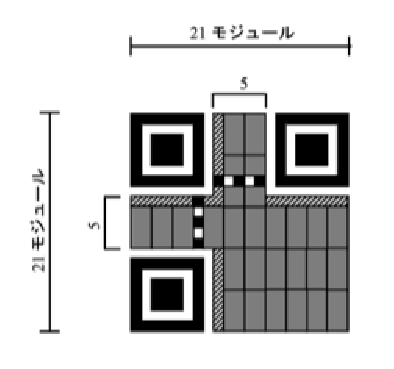
\includegraphics[width=0.5\linewidth]{pic/v1.eps}
      \caption{QRコードのバージョン1の構造}
      \label{v1}
\end{figure}

\section{作成したソフトウェア}

RS符号化は有限体の実装の容易なMaple、QRコードの生成は画像が扱いやすいJavaを使う.
ソフトウェアの実行手順を以下に示す

\begin{enumerate}
\item
文字列をMapleに入力し、RS符号が計算して得られる.
\item
得たRS符号とQRコードに含めたい目的画像をJavaに入力し、Aesthetic QRコードとして出力される.

\end{enumerate}


\begin{figure}[H]
      \centering
      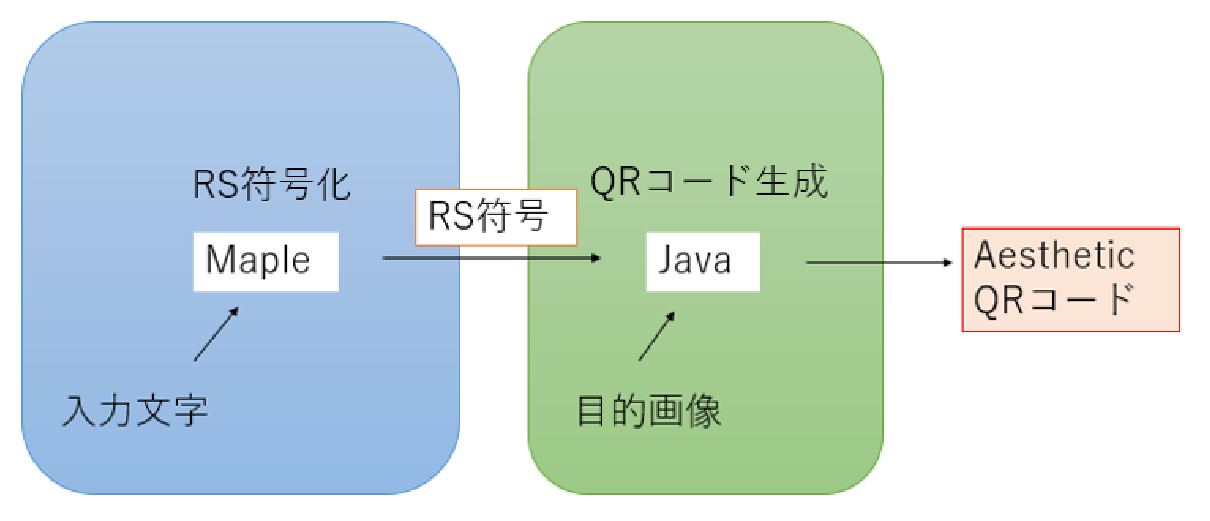
\includegraphics[width=1\linewidth]{pic/Maple_Java.eps}
      \caption{開発したソフトウェアのAesthetic QRコードの作成までの流れ}
      \label{soft}
\end{figure}

\section{評価}

画像の評価は
\begin{enumerate}
\item
目的画像の二値行列$B_{i,j}$と得られたQRコードの二値行列におけるハミング距離.
\item
$PSNR$(ピーク信号対雑音比).
\item
RS符号の生成にかかった時間.

\end{enumerate}
で行う.

ハミング距離はKuribayashiらの論文\cite{KURI}で使われている評価であり、小さければ比較対象が近いことを指す.
PSNRは画像の劣化具合を評価するのに一般的に使われているものであり、大きければ劣化具合が少ないことを指す.
RS符号の生成にかかった時間は短いほど、手軽に作成することが可能であることがわかる.
時間は10回生成して平均をとったものを評価している.

\subsection{最小ハミング距離}

2つの符号語つの符号語$a=(a_1,a_2,…,a_n)$と$b=(b_1,b_2,…,b_n)$で対応するビット(桁)で値$(0$または$1)$が異なっているビット(桁)の数をハミング距離と言い、記号で$d(a,b)$と書く.
その中でも一番ハミング距離が小さいものを最小ハミング距離と呼ぶ.

ハミング距離は2つの符号語$a=(a_1,a_2,…,a_n)$と$b=(b_1,b_2,…,b_n)$に対して以下の式で定義される.

\begin{eqnarray}
d(a,b)=\sum_{i=1}^{n}(a_{i}+b_{i})\mbox{ }(\mbox{mod } 2)
\end{eqnarray}

\subsection{$PSNR$(ピーク信号雑音比)}

$PSNR$は画質の再現性に影響を与える信号がとりえる最大の輝度と劣化をもたらすノイズの比率を示したものである.
$PSNR$は以下の式で定義される.

\begin{eqnarray}
PSNR&=&10\log{10}\frac{MAX_I^2}{MSE} \\
       &=&20\log{10}\frac{MAX_I}{\sqrt{MSE}}
\end{eqnarray}

$MAX_{I}$は画像がとりうる最大ピクセルを表す.
ピクセルの$1$サンプルが$8$ビットで表現されている場合、$MAX_{I}$は$255$である.
$MSE$(平均二乗誤差)は元画像と処理画像との差の2乗誤差である.$MSE$が小さければ小さいほど元画像に近い画像である.
$MSE$は$M \times N$の2つの画像$I、K$において、以下の式で定義される.

\begin{eqnarray}
MSE&=&\frac{1}{MN}\sum_{i=0}^{M-1}\sum_{j=0}^{N-1}[I(i,j)+K(i,j)]^2
\end{eqnarray}


\section{実験結果}

本実験でQRコードに挿入する画像は以下のみきゃん(図\ref{mican_pic})を使用した.
図\ref{fig:output_1}$\sim$\ref{fig:output_10000}はランダム法の試行回数が$N=1,10,100,1000,10000$の場合の結果(Aestheic QRコード)を表す.
実際にソフトウェアによって生成した画像が図\ref{fig:output_1}$\sim$図\ref{fig:output_10000}である.

\begin{figure}[H]
  \begin{tabular}{cc}
    %---- 最初の図 ---------------------------
    \begin{minipage}[t]{0.45\hsize}
      \centering
      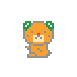
\includegraphics[width=0.5\linewidth]{pic/mican.eps}
      \caption{目的画像}
      \label{mican_pic}
    \end{minipage} &
    %---- 2番目の図 --------------------------
    \begin{minipage}[t]{0.45\hsize}
    \centering
      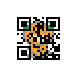
\includegraphics[width=0.5\linewidth]{pic/nomal.eps}
      \caption{目的画像にQRコードを張り付けただけのQRコード}
      \label{fig:nomal}
      \end{minipage}
  \end{tabular}
\end{figure}

\begin{figure}[H]
  \begin{tabular}{cc}
    %---- 3番目の図 ---------------------------
    \begin{minipage}[t]{0.45\hsize}
      \centering
      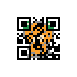
\includegraphics[width=0.5\linewidth]{pic/output_1.eps}
       \caption{$N=1$}
      \label{fig:output_1}
    \end{minipage} &
    %---- 4番目の図 --------------------------
    \begin{minipage}[t]{0.45\hsize}
     \centering
      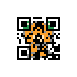
\includegraphics[width=0.5\linewidth]{pic/output_10.eps}
       \caption{$N=10$}
      \label{fig:output_10}
      \end{minipage}
  \end{tabular}
\end{figure}

 %---- 改行 ----------------------

\begin{figure}[H]
  \begin{tabular}{cc}
    %---- 5番目の図 ---------------------------
    \begin{minipage}[t]{0.45\hsize}
     \centering
      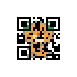
\includegraphics[width=0.5\linewidth]{pic/output_100.eps}
      \caption{$N=100$}
      \label{fig:output_100}
    \end{minipage} &
    %---- 6番目の図 --------------------------
    \begin{minipage}[t]{0.45\hsize}
     \centering
      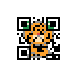
\includegraphics[width=0.5\linewidth]{pic/output_1000.eps}
       \caption{$N=1000$}
      \label{fig:output_1000}
      \end{minipage}
  \end{tabular}
\end{figure}

 %---- 改行 ----------------------

\begin{figure}[H]
    %---- 7番目の図 --------------------------
      \centering
      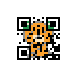
\includegraphics[width=0.25\linewidth]{pic/output_10000.eps}
       \caption{$N=10000$}
      \label{fig:output_10000}
    
\end{figure}
  %---- 図はここまで ----------------------

また、表\ref{summary}に各試行回数のハミング距離、$PSNR値$、RS符号の生成にかかった時間を表す.

\begin{table}[H]
	\caption{結果のまとめ}
	\begin{center}
  		\begin{tabular}{|c|c|c|c|c|c|} \hline
     			生成した回数 $(N) $&  $1$ & $10$ & $100$ & $1000$ & $10000$  \\  \hline
   			最小ハミング距離 &  $83$ & $69$ & $67$ & $53$ & $47$\\ \hline
			$PSNR$値$(dB)$ & $31.50$ & $31.99$ & $32.07$ & $32.82$ & $33.04$\\ \hline
			時間(秒) &  $0.0565$ & $0.4438$ & $4.2284$ & $42.0313$ & $425.5328$\\ \hline
     		\end{tabular}
  	\end{center}
  \label{summary}
\end{table}

表\ref{summary}を見ると、試行回数を増やしていくたびに評価の値が向上しており、より良いAsethetic QRコードが生成されているのがわかる.
しかし、試行回数10000回の所を見るとRS符号が生成するのにかかる時間が約7分もかかっており、あまり実用的ではない.
各評価を見ると$N=1000$の時が一番、目的画像に近い且、生成時間も短いことがわかる.

 

%%%%%%%%%%%%%%%%%%%%%%%%%%%%%%%%%%%%%%%%%%%%%%%%%%%%%%%%%%%%%%%%%%%%%%%%%%%%%%%%%%%%%%%%%%%%%%%%%%%%

\chapter{結論}
\label{chap:5}

本研究ではランダム法によって生成されるバージョン1のAesthetic QRコードのソフトウェア実装を行った.
今回は有限体の実装が容易なMapleと画像を扱いやすいJavaの2つの開発環境を使っており、二つのプログラム間のデータの転送は手動となっている.
今後の課題として、
\begin{itemize}
\setlength{\itemsep}{5mm}
 \item 今回作成したJavaのプログラムとMapleのプログラムの連結手法の検討
 \item 生成可能なAesthetic QRコードのバージョンの追加
 \end{itemize}
などが挙げられる.


\acknowledgement

本研究に際して、日々、様々なご指導をいただきました甲斐博准教授に心より感謝致します.
共同研究に際して、ご指導いただきました森井昌克教授に深謝いたします.
そして、本研究に際してご審査いただきました伊藤宏教授、稲元勉講師に感謝の意を表します.
最後に日頃から助言や励ましをいただきました諸先輩方、並びに同研究室の皆様に深く御礼を申し上げます.


\begin{thebibliography}{99}

%
\bibitem{QR}
QR code.com. http://www.qrcode.com/en.
%
\bibitem{hist}
Visualead. http://www.visualead.com.
%
\bibitem{KURI}
M. Kuribayashi and M . Morii "Aesthetic QR Code Based on Modified Systematic Encoding Function",
IEICE transactions on information and systems ,VOL.E100–D, NO.1,pp.42-51,2017.
%
\bibitem{Ikeda}
池田和興, 例題が語る符号理論, 社共立出版, 2007年
%
\bibitem{Tom}
J. Justesen and T. Hoholdt "A Course In Error-Correctiong Codes",
European Mathematical Society Publishing House, 2004.

%
%\bibitem{Sato}
%H. Sato"An introduction to the encoding-decoding algorithm of QR code - An attempt to provide an educational reading -",
%専修大学情報科学研究所所報 (76), pp37-52, 2011.
%

\bibitem{jis}
JIS X0510. http://www.jisc.go.jp/app/pager?id=2738494. 
\end{thebibliography}

\appendix

\chapter{プログラムリスト}

以下のファイルは本研究のために作成したプロフラムファイルである.
以下にソースコードを示す.
%ここまでソースコードの表示に関する設定

[Main.java]
\begin{lstlisting}
import java.awt.image.BufferedImage;
import java.io.BufferedReader;
import java.io.File;
import java.io.IOException;
import java.io.InputStreamReader;
import java.util.regex.Pattern;
import javax.imageio.ImageIO;

public class Main {
	public static int a(int c) {
		return c >>> 24;
	}
	public static int r(int c) {
		return c >> 16 & 0xff;
	}
	public static int g(int c) {
		return c >> 8 & 0xff;
	}
	public static int b(int c) {
		return c & 0xff;
	}
	public static int rgb(int r, int g, int b) {
		return 0xff000000 | r << 16 | g << 8 | b;
	}
	public static int argb(int a, int r, int g, int b) {
		return a << 24 | r << 16 | g << 8 | b;
	}
	public static void main(String[] args) throws IOException {
		// 符号全体(ここをMapleとうまく繋げたい)(今は手動でMapleで作られたものを持ってきている)
		//RS符号の入力
		InputStreamReader isr = new InputStreamReader(System.in);
		BufferedReader br = new BufferedReader(isr);

		System.out.println("RS符号を入力してください(例 11101, 1011,)");

		String str = null;
		try {
			str = br.readLine();
			br.close();
		} catch (IOException e) {
			e.printStackTrace();
		}

		Pattern p = Pattern.compile("[,\\s]+");
		String[] str_1 = p.split(str);

		int[] bit8_array = new int[str_1.length];

		for (int i = 0; i < str_1.length; i++) {
			try {
				bit8_array[i] = Integer.parseInt(str_1[i]);
			} catch (NumberFormatException e) {
				System.out.println("正しいRS符号を入力してください");
				System.out.println("プログラムを終了します。");
				return;
			}
		}

		//RS符号の確認
		System.out.println("正しくRS符号が読み込めました");

		// 10進符号→2進符号に変換
		for (int i = 0; i < bit8_array.length; i++) {
			bit8_array[i] = Integer.parseInt(String.valueOf(bit8_array[i]), 2);
		}

		// ファイル名
		String inname = "C:\\Users\\fukuda\\Desktop\\QRコード関連\\みきゃんの2値化\\使ってるの\\101_マスクパターン.png";
		String inname_2 = "C:\\Users\\fukuda\\Desktop\\QRコード関連\\みきゃんの2値化\\使ってるの\\みきゃん.png";
		String outname = "C:\\Users\\fukuda\\Desktop\\QRコード関連\\みきゃんの2値化\\使ってるの\\じっけんんn.png";
		// 画像格納クラス

		// イメージをBufferedImageへ読みこむ。
		// 以下イメージの操作はBufferedImageを利用して行う。
		BufferedImage image = ImageIO.read(new File(inname));
		BufferedImage image_2 = ImageIO.read(new File(inname_2));

		// 元イメージの幅、高さを取得。
		int w = image.getWidth();
		int h = image.getHeight();

		if (w != 21 || h != 21) {
			System.out.println("画像サイズが違います!");
			return;
		}

		// 書き込み(スパゲッティコード)(最悪だが、今は一時的にこれで)(直したい)
		int bit8;
		write_module(image, bit8_array[0], 19, 17, false);
		write_module(image, bit8_array[1], 19, 13, false);
		write_module(image, bit8_array[2], 19, 9, false);

		write_module(image, bit8_array[3], 17, 12, true);
		write_module(image, bit8_array[4], 17, 16, true);
		write_module(image, bit8_array[5], 17, 20, true);

		write_module(image, bit8_array[6], 15, 17, false);
		write_module(image, bit8_array[7], 15, 13, false);
		write_module(image, bit8_array[8], 15, 9, false);

		write_module(image, bit8_array[9], 13, 12, true);
		write_module(image, bit8_array[10], 13, 16, true);
		write_module(image, bit8_array[11], 13, 20, true);

		write_module(image, bit8_array[12], 11, 17, false);
		write_module(image, bit8_array[13], 11, 13, false);
		write_module(image, bit8_array[14], 11, 9, false);
		bit8 = bit8_array[15];
		if (bit8 % 2 != 1)
			image.setRGB(11, 4, 0x000000);
		bit8 /= 2;
		if (bit8 % 2 != 1)
			image.setRGB(12, 4, 0x000000);
		bit8 /= 2;
		if (bit8 % 2 == 1)
			image.setRGB(11, 5, 0x000000);
		bit8 /= 2;
		if (bit8 % 2 == 1)
			image.setRGB(12, 5, 0x000000);
		bit8 /= 2;
		if (bit8 % 2 == 1)
			image.setRGB(11, 7, 0x000000);
		bit8 /= 2;
		if (bit8 % 2 == 1)
			image.setRGB(12, 7, 0x000000);
		bit8 /= 2;
		if (bit8 % 2 != 1)
			image.setRGB(11, 8, 0x000000);
		bit8 /= 2;
		if (bit8 % 2 != 1)
			image.setRGB(12, 8, 0x000000);
		bit8 /= 2;
		write_module(image, bit8_array[16], 11, 0, false);

		write_module(image, bit8_array[17], 9, 3, true);
		bit8 = bit8_array[18];
		if (bit8 % 2 != 1)
			image.setRGB(9, 8, 0x000000);
		bit8 /= 2;
		if (bit8 % 2 != 1)
			image.setRGB(10, 8, 0x000000);
		bit8 /= 2;
		if (bit8 % 2 == 1)
			image.setRGB(9, 7, 0x000000);
		bit8 /= 2;
		if (bit8 % 2 == 1)
			image.setRGB(10, 7, 0x000000);
		bit8 /= 2;
		if (bit8 % 2 == 1)
			image.setRGB(9, 5, 0x000000);
		bit8 /= 2;
		if (bit8 % 2 == 1)
			image.setRGB(10, 5, 0x000000);
		bit8 /= 2;
		if (bit8 % 2 != 1)
			image.setRGB(9, 4, 0x000000);
		bit8 /= 2;
		if (bit8 % 2 != 1)
			image.setRGB(10, 4, 0x000000);
		bit8 /= 2;
		write_module(image, bit8_array[19], 9, 12, true);
		write_module(image, bit8_array[20], 9, 16, true);
		write_module(image, bit8_array[21], 9, 20, true);

		write_module(image, bit8_array[22], 7, 9, false);

		write_module(image, bit8_array[23], 4, 12, true);

		write_module(image, bit8_array[24], 2, 9, false);

		write_module(image, bit8_array[25], 0, 12, true);

		//目的画像にQRコードをかぶせる
		QRcode_to_Mican(image, image_2, h, w);

		// イメージをファイルに出力する
		ImageIO.write(image, "png", new File(outname));

		// 正常に終了
		System.out.println("正常にAestheticQRコードが出来ました");
	}

	public static void write_module(BufferedImage writebuf, int bit8, int origin_x, int origin_y, boolean isUp) {
		int sin_y;
		sin_y = isUp ? -1 : 1;

		for (int offset_y = 0; offset_y < 4; offset_y++) {
			for (int offset_x = 0; offset_x < 2; offset_x++) {
				if (((bit8 % 2) ^ ((origin_y + sin_y * offset_y) % 2)) == 0) {
					writebuf.setRGB(origin_x + offset_x, origin_y + sin_y * offset_y, 0x000000);
				}
				bit8 /= 2;
			}
		}
	}

	//
	public static void QRcode_to_Mican(BufferedImage Read_QRcode, BufferedImage Read_QRcode_2, int h, int w) {

		for (int x = 0; x < h; x++) {
			for (int y = 0; y < w; y++) {
				int c = Read_QRcode.getRGB(x, y);
				int c2 = Read_QRcode_2.getRGB(x, y);

				// モノクロに変換
				int mono = (int) (0.299 * r(c) + 0.587 * g(c) + 0.114 * b(c));
				if (mono == 0) {
					Read_QRcode.setRGB(x, y, 0x000000);//QRコードの部分(黒にする)

				} else {
					Read_QRcode.setRGB(x, y, c2);//目的画像の部分
				}
			}

		}
	}
	
}
\end{lstlisting}

\newpage

[Binarization.java]
\begin{lstlisting}
import java.awt.image.BufferedImage;
import java.io.File;
import java.io.IOException;
import javax.imageio.ImageIO;

public class Binarization {

	public static int a(int c) {
		return c >>> 24;
	}
	public static int r(int c) {
		return c >> 16 & 0xff;
	}
	public static int g(int c) {
		return c >> 8 & 0xff;
	}
	public static int b(int c) {
		return c & 0xff;
	}
	public static int rgb(int r, int g, int b) {
		return 0xff000000 | r << 16 | g << 8 | b;
	}
	public static int argb(int a, int r, int g, int b) {
		return a << 24 | r << 16 | g << 8 | b;
	}

	public static void main(String[] args) throws IOException {

		// ファイル名
		String inname = "C:\\Users\\fukuda\\Desktop\\QRコード関連\\みきゃんの2値化\\使ってるの\\みきゃん.png";
		String outname = "C:\\Users\\fukuda\\Desktop\\QRコード関連\\みきゃんの2値化\\使ってるの\\みきゃん_2値化.png";

		// 画像格納クラス

		// イメージをBufferedImageへ読みこむ。
		// 以下イメージの操作はBufferedImageを利用して行う。
		BufferedImage readImage = ImageIO.read(new File(inname));

		// モノクロに変換
		// 元イメージの幅、高さを取得。
		int w = readImage.getWidth();
		int h = readImage.getHeight();

		// 変換結果を書き込むBufferedImageを作成する。
		// サイズは元イメージと同じ幅、高さとする。
		BufferedImage write = new BufferedImage(w, h, BufferedImage.TYPE_INT_RGB);

		//ヒストグラムの初期化
		int hist[] = new int[256];

		// 1ピクセルづつ処理を行う
		for (int y = 0; y < h; y++) {
			for (int x = 0; x < w; x++) {
				// ピクセル値を取得
				int c = readImage.getRGB(x, y);
				// 0.299や0.587といった値はモノクロ化の定数値
				int mono = (int) (0.299 * r(c) + 0.587 * g(c) + 0.114 * b(c));
				write.setRGB(x, y, rgb(mono, mono, mono));
			}
		}

		//グレースケールのヒストグラムを作成
		for (int y = 0; y < h; y++) {
			for (int x = 0; x < w; x++) {
				int c = readImage.getRGB(x, y);
				int mono = (4899 * r(c) + 9617 * g(c) + 1868 * b(c) + 8192) >> 14;
				hist[mono]++;
			}
		}

		//閾値を設定(色変換手法)
		double ave = 0;
		for (int y = h / 4; y < h * 3 / 4; y++) {
			for (int x = w / 4; x < w * 3 / 4; x++) {
				int c = readImage.getRGB(x, y);
				int mono = (int) (0.299 * r(c) + 0.587 * g(c) + 0.114 * b(c));
				ave += mono;
			}
		}
		ave *= 4;
		ave /= h;
		ave /= w;

		//System.out.println(ave);(確認用)

		//閾値を元に2値化する
		for (int y = 0; y < h; y++) {
			for (int x = 0; x < w; x++) {
				int c = readImage.getRGB(x, y);
				int mono = (int) (0.299 * r(c) + 0.587 * g(c) + 0.114 * b(c));
				if (mono < ave) {
					write.setRGB(x, y, 0x000000);//黒へ

				} else {
					write.setRGB(x, y, 0xFFFFFF);//白へ
				}
			}
		}

		// イメージをファイルに出力する
		ImageIO.write(write, "png", new File(outname));
		// 正常に終了
		System.out.println("OK!");

	}

}

\end{lstlisting}



\newpage

[MSE\_PSNR.java]
\begin{lstlisting}

import java.awt.Color;
import java.awt.image.BufferedImage;
import java.io.File;
import java.io.IOException;
import javax.imageio.ImageIO;

public class MSE_PSNR {
	public static void main(String[] args) {
		try {
			//比較する画像のパスを指定
			String Comparison_1 = "C:\\Users\\fukuda\\Desktop\\QRコード関連\\みきゃんの2値化\\使ってるの\\みきゃん.png";
			String Comparison_2 = "C:\\Users\\fukuda\\Desktop\\QRコード関連\\みきゃんの2値化\\使ってるの\\出力_10000.png";

			//画像ファイルを読み込む
			BufferedImage img_1 = ImageIO.read(new File(Comparison_1));
			BufferedImage img_2 = ImageIO.read(new File(Comparison_2));

			//もろもろの値の初期化
			double sum = 0;
			double ave_1 = 0;
			double ave_2 = 0;
			double max_1 = 0;
			double max_2 = 0;
			double min = 1000000;

			//画像の縦、横の長さを取得
			int h = img_1.getHeight();
			int w = img_1.getWidth();

			//MES値を計算
			for (int i = 0; i < w; i++) {
				for (int j = 0; j < h; j++) {
					Color color_1 = new Color(img_1.getRGB(i, j));
					Color color_2 = new Color(img_2.getRGB(i, j));
					ave_1 = (color_1.getRed() + color_1.getGreen() + color_1.getBlue());
					if (ave_1 > max_1) {
						max_1 = ave_1;
					}
					ave_2 = (color_2.getRed() + color_2.getGreen() + color_2.getBlue());
					if (ave_2 > max_2) {
						max_2 = ave_2;
					}
					sum += Math.pow(color_1.getRed() - color_2.getRed(), 2)
							+ Math.pow(color_1.getGreen() - color_2.getGreen(), 2)
							+ Math.pow(color_1.getBlue() - color_2.getBlue(), 2);
				}
			}

			sum /= 3;
			sum /= h;
			sum /= w;

			if (min > sum) {
				min = sum;
			}

			//MSE値を出力
			System.out.println("MSE");
			System.out.println(sum);

			//PSNR値を計算
			double a = Math.sqrt(sum);
			double positiveValue1000 = max_2 / a;

			//PSNR値を出力
			System.out.println("PSNR");
			System.out.println(20 * Math.log(positiveValue1000));

		} catch (IOException e) {
			e.printStackTrace();
		}
	}
}
\end{lstlisting}

\newpage

[Random\_RScode.mw]
\begin{lstlisting}
restart;
 
ts := time(); 

#ガロア体GF(2^8)の定義
G8 := GF(2, 8, alpha^8+alpha^4+alpha^3+alpha^2+1); 

a := G8:-ConvertIn(alpha); 

#QRコード、バージョン1、誤り訂正レベルMの定義(https://sites.google.com/a/osshc.co.cc/web/studies/it/qr)
#埋め草シンボルの数khatの定義

n := 26; k := 16; khat := 9; 

#誤り訂正コード語数10の生成多項式GPの定義(a^t の指数 t のみを並べたベクトルで表現、https://sites.google.com/a/osshc.co.cc/web/studies/it/qr)

GP := Vector(n-k+1, [0, 251, 67, 46, 61, 118, 70, 64, 94, 32, 45]); 

#情報シンボルFの定義(FP は a^t の 指数 t のみを並べたベクトル(t=-1 のときはシンボルが0を表す)、https://sites.google.com/a/osshc.co.cc/web/studies/it/qr)

#FUKUDAのコード語[5, 194, 45, 10, 152, 16, conv[0], 49, 252, 29, 217, 113, 168, 24, 196, 216]
FP := Vector(k, [5, 194, 45, 10, 152, 16, -1, 122, 100, 122, 100, 122, 100, 122, 100, 122]); 

F := Vector(k); 

for i to k do 
	if FP[i] >= 0 then 
		F[i] := G8:-`^`(a, FP[i]) 
	else 
		F[i] := G8:-input(0) 
	end if
end do; 

#ハミング距離の比較対象

Mican := [10001100, 10101101, 110000, 10011011, 11111, 11111100, 10001111, 11001000, 11000011, 11, 11000000, 11000011, 10100011, 11111011, 101111, 10001100, 10110101, 11000110, 110011];

#min_distanceの初期化
min_distance := 8*n; 

#ここから繰り返す
for REPEAT to 1 do

#生成行列Gの作成
G := Matrix(k, n); 

for i to k do 
	for j to n do 
		G[i, j] := G8:-input(0) 
	end do 
end do; 

for i to k do 
	for j to 11 do 
		G[i, i-1+j] := G8:-`^`(a, GP[j]) 
	end do 
end do; 

#符号に現れる、情報シンボルの位置(1~(k-khat))と埋め草シンボルの位置(k-khat~nのどこかのkhat個)を, deltaで定義
delta := Vector(k); 

for i to k-khat do
	delta[i] := i 
end do; 

myrand := rand(k-khat+1 .. n); 
myset := {}; 
while nops(myset) <> khat do 
	myset := myset union {myrand()} 
end do; 

mylist := convert(myset, list); 
for i to khat do 
	delta[i+k-khat] := mylist[i] 
end do; 

#掃き出し法によりGをランダム法で使う(I|P)に変形
#Iの後半の列はPのどこかの列にランダムに入る

for i to k do 
	inv := G8:-inverse(G[i, delta[i]]); 
	for j to n do 
		G[i, j] := G8:-`*`(inv, G[i, j]) 
	end do; 
	for l to i-1 do 
		tmp := G[l, delta[i]]; 
		for j to n do 
			G[l, j] := G8:-`-`(G[l, j], G8:-`*`(tmp, G[i, j])) 
		end do 
	end do; 
	for l from i+1 to k do 
		tmp := G[l, delta[i]]; 
		for j to n do 
			G[l, j] := G8:-`-`(G[l, j], G8:-`*`(tmp, G[i, j])) 
		end do 
	end do 
end do; 

#符号の計算 C=F*G
C := Vector(n); 

for i to n do 
	C[i] := G8:-input(0); 
	for j to k do 
		C[i] := G8:-`+`(C[i], G8:-`*`(F[j], G[j, i])) 
	end do 
end do; 

#符号 C(Rx) を表示してみる
Rx := [seq(convert(G8:-output(C[i]), binary, decimal), i = 1 .. n)]; 

#ハミング距離の計算
distance := 0; 

for i to nops(Mican) do 
	number_rx := Rx[nops(Rx)-nops(Mican)+i]; 
	number_mi := Mican[i]; 
	for j from 1 to 8 do 
		if number_rx mod 10 != number_mi mod 10 then 
			distance := add(distance, k = 1 .. 1)+1 
		end if; 
		number_rx := (add(number_rx, k = 1 .. 1)-add(number_rx mod 10), k = 1 .. 1))*(1/10); 
		number_mi := (add(number_mi, k = 1 .. 1)-add(number_mi mod 10, k = 1 .. 1))*(1/10) 
	end do 
end do; 

#最小ハミング距離を求める
if distance < min_distance then 
	min_distance := distance; 
	kekka := Rx 
end if 

#繰り返し終了
end do; 

#計算時間の表示
print(time()-ts); 

#最小ハミング距離の表示
print(min_distance); 

#RS符号の表示
print(kekka)
\end{lstlisting}

\end{document}
